\chapter{Kapitel 4}

\section{Dateien}

Ein Dateisystem ist nötig aus drei wesentlichen gründen:

\begin{enumerate}
    \item Es muss möglich sein, sehr große Mengen von Informationen zu speichern, für
          welche der Hauptspeicher nicht ausreicht.
    \item Informationen müssen die Terminierung von Prozessen überstehen. Wenn Daten also
          erzeugt werden und der PC neugestartet wird, müssen diese Daten weiterhin
          erhalten bleiben.
    \item Es muss für mehrere Prozesse möglich sein, gleichzeitig auf die
          In\-for\-mation\-en zuzugreifen. Mehrere Prozesse können beispielswesie auf die
          selben Dateien zugreifen.s
\end{enumerate}

Eine Datei ist eine logische Information von Daten.

Dateien werden vom Betriebssystem verwaltet. Der teil des Betriebssystems, der
für die Dateien zuständig ist, wird Dateisystem genannt. Beim entwurf von
Dateisystemen müssen folgende Themen betrachtet werden:

\begin{itemize}
    \item Strukturierung
    \item Benennung
    \item Zugriff
    \item Benutzung
    \item Schutz
\end{itemize}

\subsection{Benennung}

Eine Datei ist ein Abstraktionsmechanismus für Daten. Es sollen keine Kentnisse
über die Implementierung vorausgesetzt werden. Informationen wie und wo Dateien
gespeichert sind, sollten irrelevant sein.

Regeln für die Benennung von Dateien variieren. Uniter UNIX dürfen Dateien bis
zu 255 Zeichen lang sein. Außerdem wird in UNIX zwischen Groß und
Klein-schreibung unterschieden. Unter Windoes ist Groß- und Kleinschreibung
irrelevant. Unter Dos durfte der Name nur 1-8 Zeichen und die Dateiendung nur
1-3 Zeichen lang sein.

Unter UNIX ist die verwendung von einer oder mehrerer Dateiendungen zulässig.
Beispielsweise ist der Name \texttt{index.html.zip} in UNIX zulässig.
Datei\-namens\-er\-weiterungen sind also nur Konvention. Beispielsweise kann
die Datei \texttt{file.txt} genausogut eine Ausführbare Datei sein. Trotzdem
erwarten einige Programme eine gewisse Dateiendung. Der C-Compiler erwartet
eine Datei mit der Endung \texttt{.c}.

Unter Windows haben Dateiendungen eine feste Wirkung. Die Dateiendung legt hier
fest, mit welchem Programm dateien beispielswesie geöffnet werden sollen.

\subsection{Dateistrukturen}

Dateien müssen strukturiert werden. Hierfür gibt es viele möglichkeiten.

Eine Datei ist eine Folge von Bytes. Das Betriebssystem kennt den Inhalt nicht.
Die Interpretation der Daten geschieht auf Anwendungsebene.

Die Dateien besitzen eine Folge von Datensätzen fester größe. Beispielsweise
besteht eine Datei aus n Datensätzen, welche je m bytes beinhalten dürfen.

Eine Datei besteht aus einem Baum von Datensätzen mit unterschiedlicher länge.
Hier entscheidet nicht der Benutzer, welche Struktur die Dateien haben, sondern
das Betriebssystem tut dies.

\subsection{Dateitypen}

Reguläre Dateien sind entweder ASCII-Dateien, also Dateien die Lesbar,
editirbar und Druckbar sind, oder Dateien können Binär Dateien sein. Sie
enthalten Prozessorinstruktionen oder Binärdekodierte Daten. In UNIX haben
Ausführbare Programme die Struktur Kopf, Text, Daten, Relokationsbit,
Symboltabelle.

\subsection{Dateizugriff}

Wenn auf Dateien zugegriffen werden soll, gibt es zwei Möglichkeiten:

\begin{itemize}
    \item Sequentieller Zugriff: Es wird auf eine Datei zugegriffen und Die gesammte
          Datei wird gelesen, bis die gewünschte Stelle gefunden wird. Dies wird heute
          nicht mehr gemacht.
    \item Wahlfreier Zugriff: Es kann in beliebiger Reihenfolge auf Bytes oder Sätze in
          der Datei zugegriffen werden.
\end{itemize}

Der Lese/Schreibe Kopf muss über den \texttt{seek} Systemaufruf an die
gewünschte stelle geschoben werden.

\subsection{Dateiattribute}

In den Dateiattrubiten sind Informationen wie Besitzer, Ersteller, Schutzinfos
und vieles weitere gespeichert.

\subsection{Dateioperationen}

Das Betriebssystem muss die Ressource Datei verwalten. Es stellt viele
Systemaufrufe für Dateien bereit.

\begin{itemize}
    \item create: es wird eine neue Datei ohne Daten erzeugt. Hier werden, obwohl kein
          Inhalt in der Datei ist, einige Dateiattribute gesetzt.
    \item delete: löscht eine Datei
    \item open: Öffnet eine Datei. Hier muss festgelegt werden, ob die Datei zum lesen
          und oder schreiben geöffnet werden soll.
    \item close: schließt eine Datei. Gibt den Tabellenplatz der Datei wieder frei.
    \item read: von der AKtuellen Position wird gelesen
    \item write: von der aktuellen Position wird geschrieben
    \item append: es wird hinten an der Datei etwas angefühgt.
    \item seek: Ausgabe des SChreib/Lesekopf Position
    \item Get attributes: Prozess benötigt die Dateiattribute. Beispiel make
    \item Set attributes: Prozesse können eigene Attribute setzen
    \item rename: Dateiname wird geändert
\end{itemize}

Es gibt noch sehr viele weitere Systemaufrufe für Dateien.

\section{Verzeichnisse}

Ein Verzeichnis ist eine Ordnungsstruktur auf das Dateisystem. Es gibt
Dateisysteme, die keine Ordnungsstruktur hatten, z.B: frühere PCs, eingebettete
Systeme oder einige tragbare Musikplayer. Dies hat den Vorteil dass das
Dateisystem schnell und einfach ist.

\subsection{Hierarchie Verzeichnissysteme}

Gängige Verzeichnishierarchien können Dateien in Ordnern in Ordnern in
Ordnern... haben. Dies ist eine Baumstruktur. Wenn auf eine Datei zugegriffen
werden soll, dann muss der gesammte Pfad vom Wurzelverzeichnis angegeben
werden. Unterschiedliche Betriebssysteme haben unterschiedliche Pfadangaben.
Uniter UNIX wird mit dem \texttt{/} (slash) zwischen Unterverzeichnissen
getrennt, unter Windows wird das \texttt{\\} (backslash)
verwendet.

Mit Relativen Pfaden kann im aktuellen Arbeitsverzeichnis eine Datei genutzt
werden \texttt{./ast/mailbox} sucht im Aktuellen Verzeichnis nach der Datei
\texttt{ast/mailbox}. \texttt{..} bezieht sich auf das übergeordnete
Verzeichnis.

\subsection{Operationen auf Verzeichnisse (Prüfungshinweis)}

Für Verzeichniswe stellt das Betirebssystem einge Systemaufrufe bereit

\begin{itemize}
    \item create: es wird ein neues Verzeichnis erzeugt.
    \item delete: Es wird ein Verzeichnis gelöscht
    \item opendir: es wird ein Verzeichnis geöffnet.
    \item closedir: Es wird ein Verzeichnis geschlossen
    \item ....: Liest die nächste Datei aus dem geöffneten Verzeichnis
    \item rename: benennt ein Verzeichnis um
    \item link: Linken erlaubt es, eine Datei in mehr als einem verzeichnis erscheinen zu
          lassen
    \item unlink: hebt ein Link auf.
\end{itemize}

Es gibt zwei Arten von Links (prüfungsrelevant):

\begin{itemize}
    \item Symbolische Links: Wenn auf eine Datei zugegriffen wird, wird der Pfad der
          Datei einfach mit dem Pfad der originalen Datei verwendet.
    \item Harte Links: Verweist auf den Inode des Dateisystems. Es kann sofort auf die
          Datei zugegriffen werden, ohne dass auf den Verzeichnisbaum zugegriffen werden.
          Dies funktioniert nicht über das Netzwerk.
\end{itemize}

\section{Implementierung von Dateisystemen}

\subsection{Layout eines Dateisystems}

Das Dateisystem wird auf der Festplatte gespeichert. Alle Informationen, welche
nebnötigt werden, um das Dateisystem aufzubauen muss auch auf der Festplatte
gespeichert werden. Es kann nichts im Haupspeicher gespeichert bleiben, da
dieser leer ist, wenn der Rechner aus ist.

Die Festplatte wird in Partitionen aufgeteilt, welche voneinander unabhängige
Dateisysteme sind. In jeder Partition kann ein unterschiedliches Dateisystem
vorhanden sein. Wie diese PArtitionen aufgebaut sind, steht in dem Sogenannten
Sektor 0, dem Master Book Record (MBR). Am Ende des MBR steht die
Partitionstabelle mit anfangs und endadresse jeder Partition. Eine dieser
Partition ist aks aktiv makiert, die Boot-Partition.

Beim Hochfahren des Rechners liest das BIOS das MBR ein. Dieses lokalisiert als
erstes die Aktive Partition, liest den ersten Block ein (den Boot-Block) und
führt ihn aus. Das Programm im Boot-Block lädt das Betriebssystem, das in der
Partition gespeichert ist. \textbf{Jede} Partition beginnt mit einen
Boot-Block.

Im Super Block, welcher sich unmittelbar nach dem Boot Block befindet, werden
Schlüsselparameter des Dateisystems geladen. Die Freispeicherverwaltung gibt
an, welche stellen im Speicher noch frei sind. Die I-Notes geben die
vorhandenen Dateien an. Das Wurzelverzeichnis gibt das Wurzelverzeichnis des
Dateisystems an.

\subsection{Implementierung von Dateien}

Das Hauptproblem bei der Implementierung ist die Allokation und Freigabe von
Plattenblöcken. Es muss geschaut werden, welche Plattenblöcke frei sind und
welche nicht. Hierfür gibt es einige verfahren

\subsubsection{Zusammenhängende BElegung}

Jede Datei wird als eine Zusammenhängende MEnge von Plattenblöcken gespeichert.
Es muss hier nur der vorderste Plattenblock gemerkt werden, da alle
nachfolgenden Blöcke zu der selben Datei gehören. Die Leseperformance ist hier
ausgezeichnet.

Der Nachteil an diesem System sit, dass Dateien nur gespeichert werden können,
wenn man genau weiß wie groß diese sind. Bei der Löschung von Dateien entstehen
löcher, wodurch die Interne Fragmentierung wieder ein Problem wird.

Dieses Verfahren wird heute bei CDs, DVDs und Blu-rays verwendet, da der Inhalt
dieser idr. nciht verändert wird.

\subsubsection{Belegung durch verkettete Listen}

Es existiert in jedem Block ein ZEiger auf den folgenden Block. Es kann jeder
Block in jeder beliebigen Reihenfolge verwendet werden. Es gibt keine INterne
Fragmentierung. Es muss nur der Start Block gemerkt werden.

Für Zufällige zugriffe ist dieses verfahren jedoch sehr langsam. Wenn an die
letzte Stelle gesprungen werden will, muss durch die gesammte Liste gesprungen
werden.

\subsection{Belegung durch Verkettete Liste mit Tabelle im Arbeitsspeicher}

Es werden die Zeiger jedes Plattenblocks in einer Datei-allokations-tabelle
(FAT) im arbeitsspeicher gespeichert. Zufälliger Zugriff ist heir einfach, da
die Tabelle sich im Arbeitsspeicher befindet. Der Verzeichniseintrag besteht
hier nur aus der Startblocknummer.

Jedoch kann die Tabelle sehr groß werden. Bei beispielsweise eienr 1TB
festplatte, 4KB Blöcken und 3 bytes je Eintrag führt dies zu einer 3GB Tabelle
im Hauptspeicher.

\subsubsection{I-Nodes}

Die I-Nodes werden in UNIX verwendet. In I-Nodes werden Attribute eienr Datei
gespeichert. Sie enthält auch die Plattenadressen der Datei. Wenn eine I-Note
nicht reicht, dann wird auf eine weitere I-Node verwiesen.

Ähnlich funktioniert auch das NTFS Dateisystem von Windows.

\subsection{Implementierung von Verzeichnissen}

\subsubsection{Verzeichnisse unter MS-DOS}

Unter MS-Dos ist ein Verzeichniseintrag wie folgt aufgebaut: die ersten 8 Bit
sind für den Dateinamen reserviert. Die nächsten 3 für die Erweiterun..

\subsubsection{Verzeichnisse unter UNIX}

Ein Verzeichniseintrag ist aufgebaut mit dem Dateinamen und der I-Node nummer.
Die ersten 2 byte stehen für die I-Node nummer. die verbleibenden 14 Byte für
den Dateinamen.

Wird beispielsweise nach dem Verzeichnis usr gesucht, so wird das
Wurzelverzeichnis durchsucht. Dies kann beispielsweise zu der I-Node Nummer 6
führen. In diesem steht neben einigen Attributen der Block 132. Der Block 132
wird dann nach ast durchsucht. Dort steht, dass der Inhalt im I-Node 32 zu
finden ist.

\section{Dateisyystemverwaltung und -optimierung}

Dateisysteme teilen Dateien in Blöcke mit fester Größe auf, welche nicht
zusammen gehören müssen. Festplatten sind Organisiert in:

\begin{itemize}
    \item Sektoren (B)
    \item Spuren (A)
    \item Zylindern
    \item Blöcken (C)
    \item Clustern (D)
\end{itemize}

\begin{figure}[h!]
    \centering
    \begin{minipage}{0.48\textwidth}
        \centering
        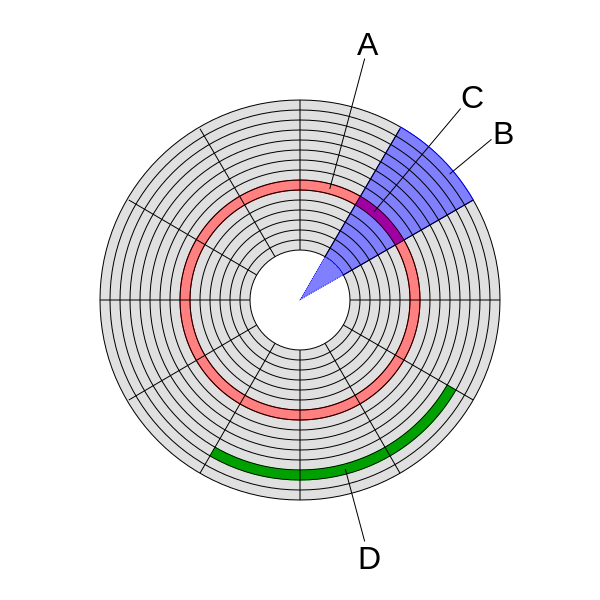
\includegraphics[width=\linewidth]{disk_structure.png}
    \end{minipage}\hfill
    \begin{minipage}{0.48\textwidth}
        \centering
        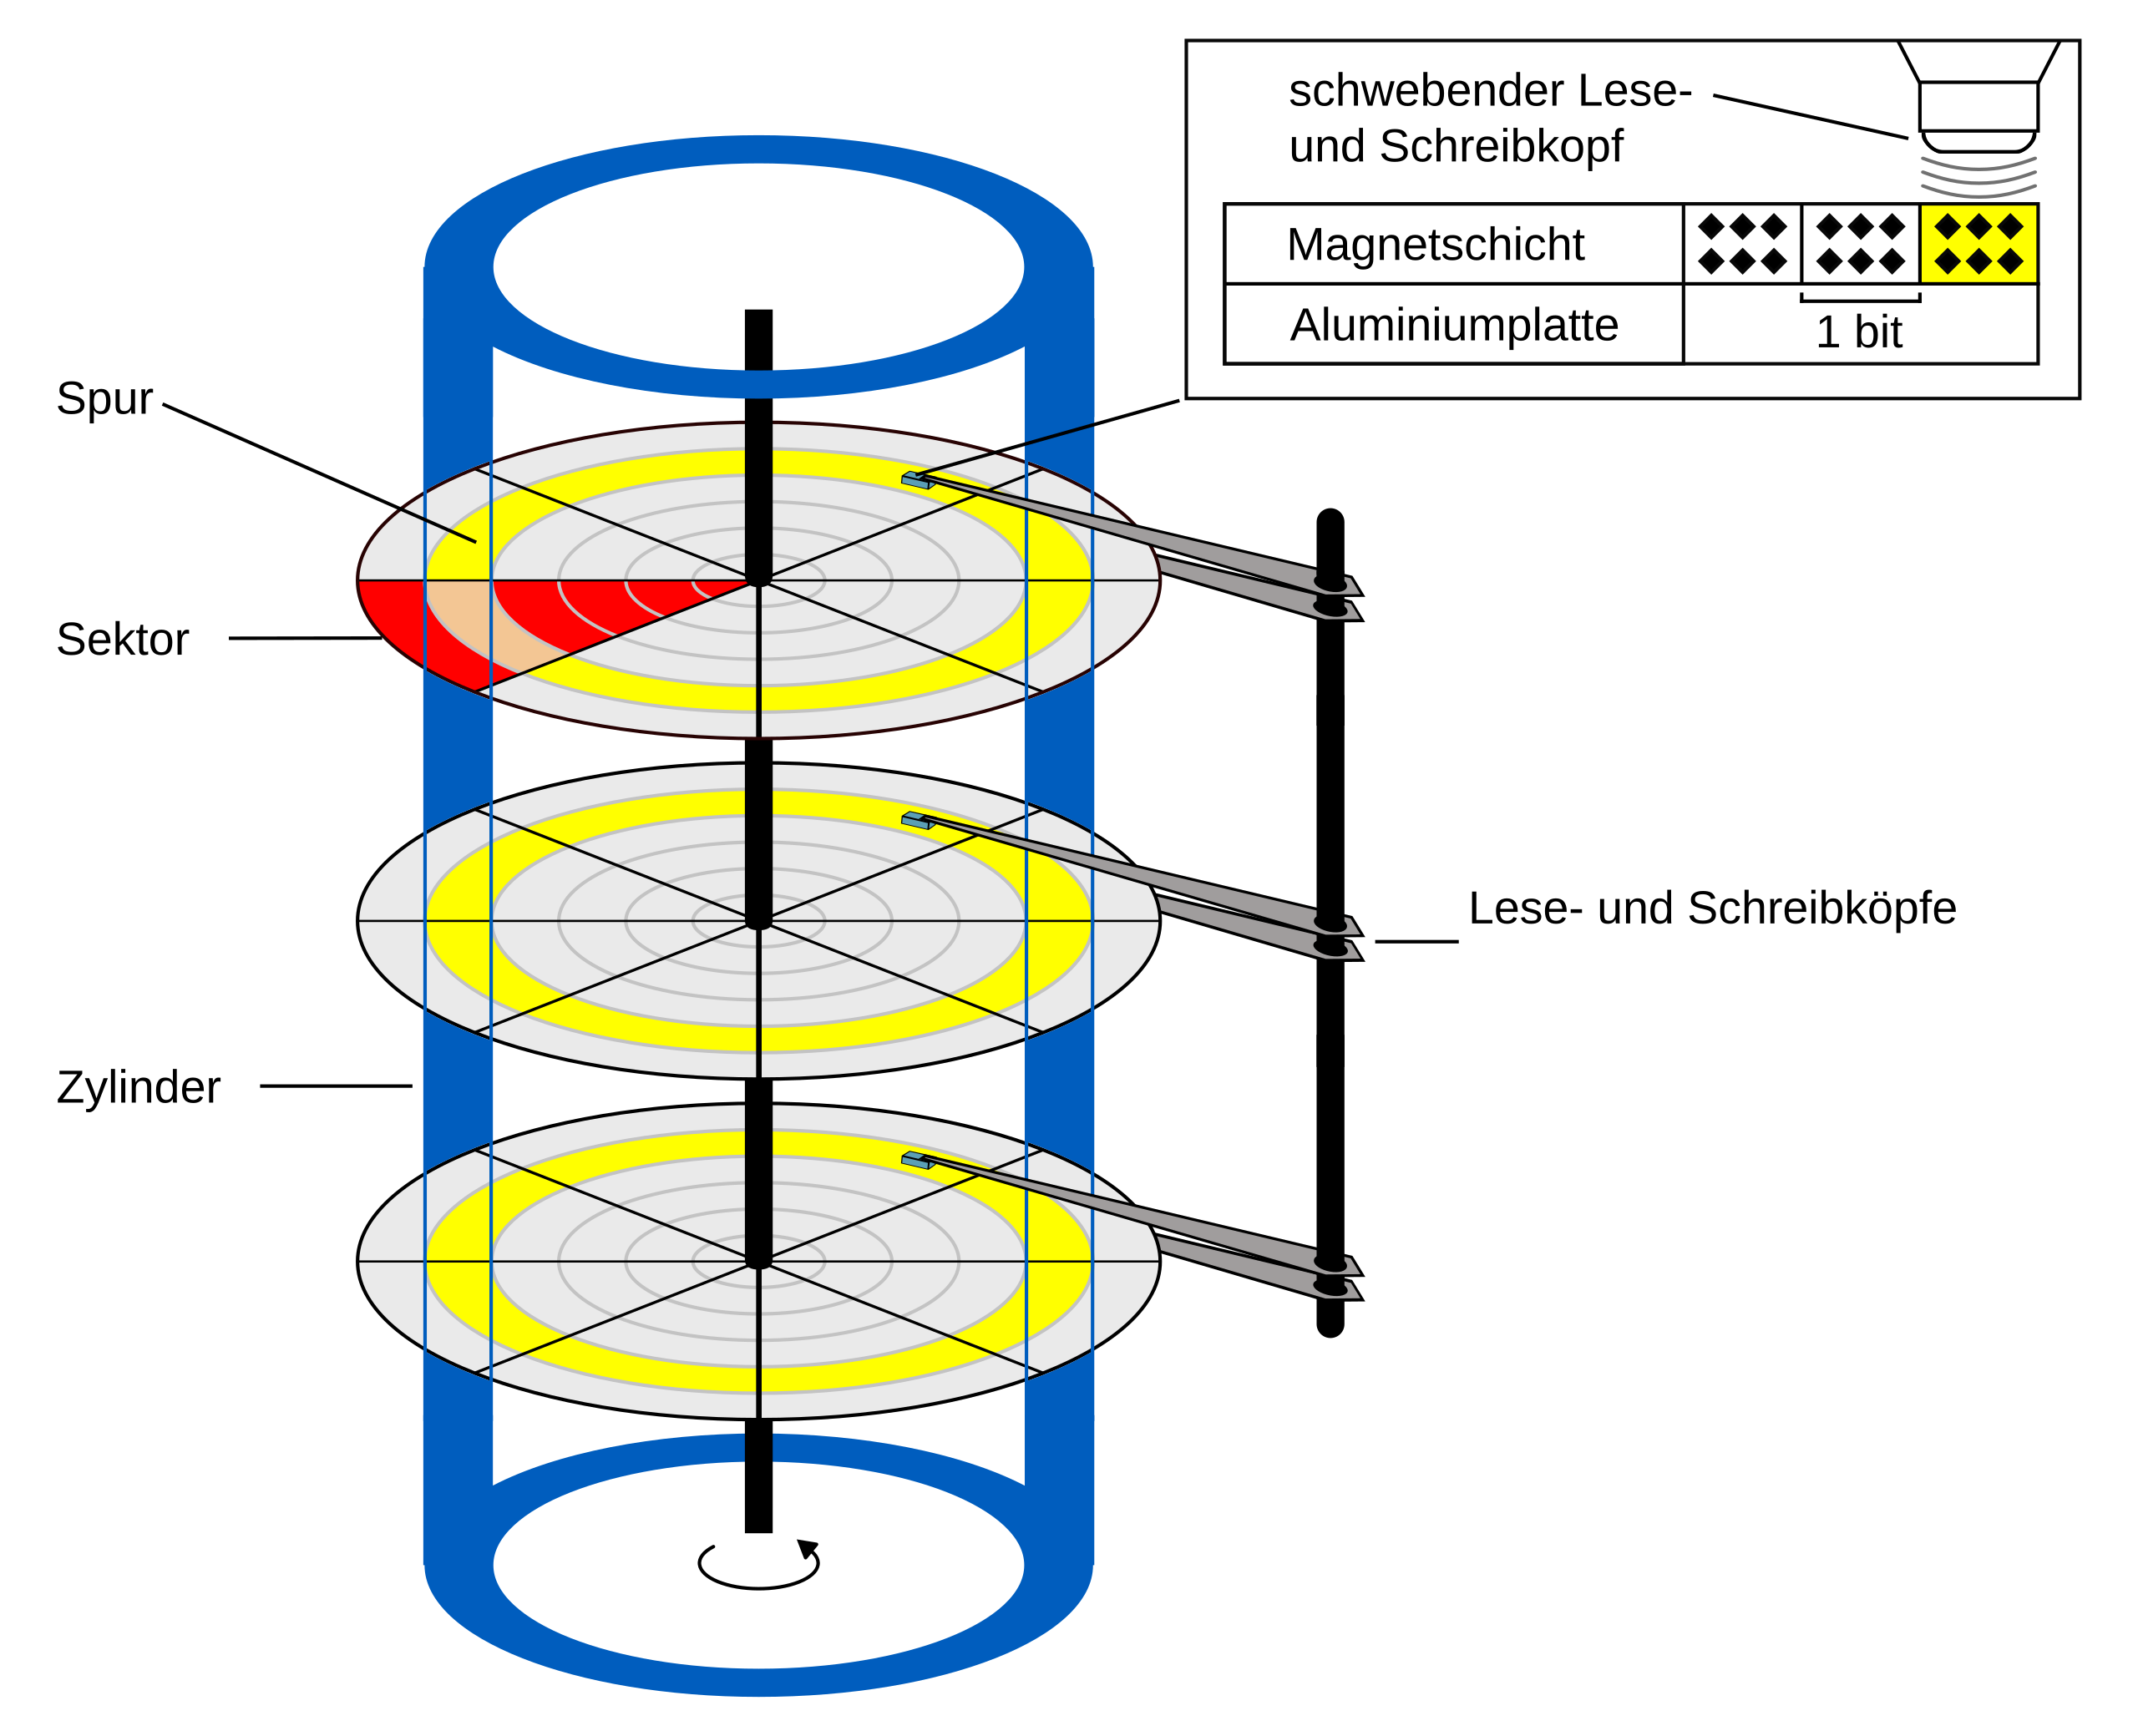
\includegraphics[width=\linewidth]{disk_structure2.png}
    \end{minipage}
\end{figure}

Werden große Allokationseinheiten verwendet (wie z.B. einen Zylinder)
verschwendet die Speicherung von wenig Daten, wie einem einzigen Byte
offensichtlich sehr viel Plattenplatz. Werden hingegen kleine
Allokationseinheiten verwendet, so dauert das Lesen sehr lange. Beim Lesen von
Dateien aus vielen Blöcken muss zunächst gewartet werden, bis der Schreib/Lese
Kopf an der richtigen Position ist.

2005 lag die mittlere Dateigröße bei 2475 Byte. Bei 4-KB Blöcken werden also 93\%
der Plattenblöcke von 10 \% der Daten belegt. Ein wenig Platzverschwendung bei jeder
Datei fällt kaum ins Gewicht, da die Platte mit wenigen großen Daten gefüllt ist.
Selbst eine Verdopplung des Platzes, den die kleinsten 90\% der Daten verbrauchen,
würde kaum bemerkt werden.

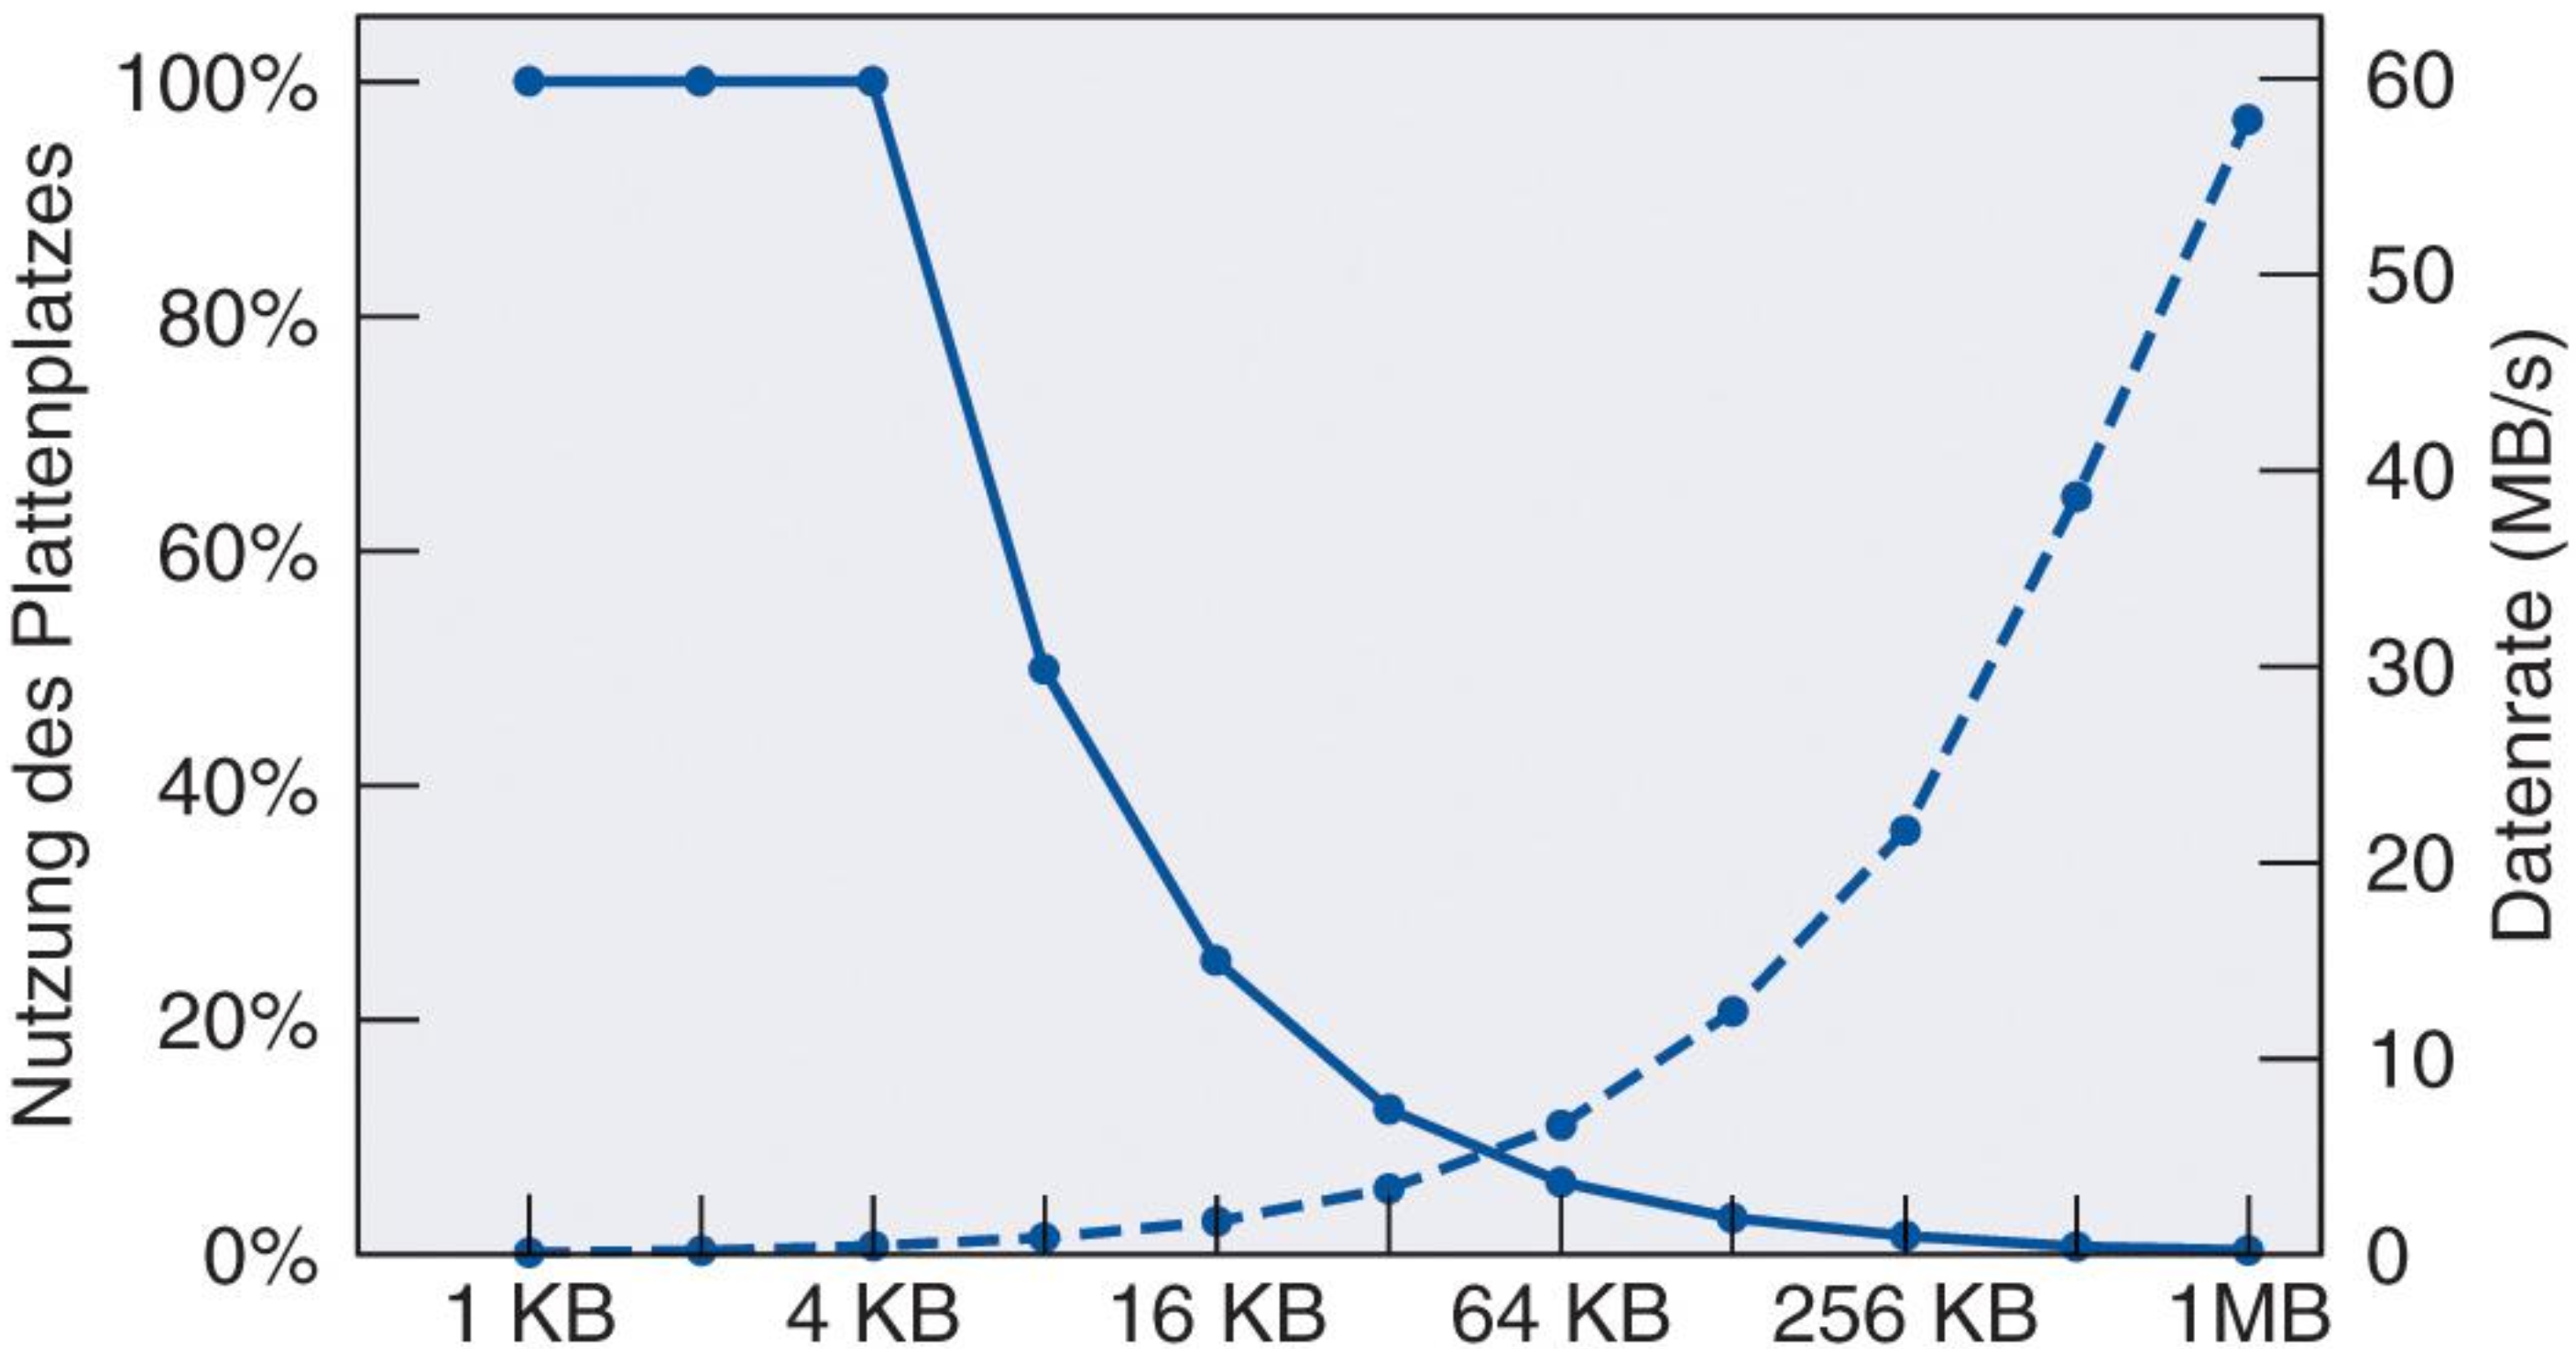
\includegraphics[width=\linewidth]{disk_speed.png}

Die Abbildung verdeutlicht den zentralen Zielkonflikt: Die
\textbf{durchgezogene Linie} zeigt, dass die Platzeffizienz bei kleinen Blöcken
am besten ist. Die \textbf{gestrichelte Linie} zeigt jedoch, dass die Datenrate
(Geschwindigkeit) mit größeren Blöcken stark zunimmt.

Dieser Kompromiss hat sich über die Zeit verschoben:
\begin{itemize}
    \item \textbf{Früher (1-4 KB Blöcke):} Speicher war teuer und knapp. Man opferte
          Geschwindigkeit, um durch kleine Blöcke Platz zu sparen.
    \item \textbf{Heute (z.B. 64 KB Blöcke):} Speicher ist günstig und im Überfluss
          vorhanden. Man priorisiert die hohe Geschwindigkeit und nimmt dafür die
          Platzverschwendung bei kleinen Dateien (sog. interne Fragmentierung) in Kauf.
\end{itemize}

\subsection{Verwaltung freier Blöcke}

\subsubsection{Über Verkettete Liste}

Werden Blöcke in einer Verketteten Liste organisiert, erhält jeder Plattenblock
eine Freie Plattenblocknummer. Bei einer Blockgröße von einem KB und
32-Bit-Blocknummern gibt es 255 freie Blöcke. 1 Verweis aus nächsten Block. Da
nur freie Blöcke verwendet werden, wird kein Plattenplatz verschwendet. Bei
einer 1TB-Festplatte gibt es ca. eine Milliarde Blöcke. ca. 4 Millionen Blöcke
werden als Freispeicher benötigt.

\subsubsection{Bitmap}

Eine Platte mit \texttt{n} Blöcken benötigt \texttt{n} Bit. Ein Freier Block
wird über eine 1 definiert, ein nicht leerer über eine 0 (oder Umgekehrt). Eine
1TB Festplatte benötigt eine Milliarde Bit, also 130.000 1KB-Blöcke für die
Speicherung der Bitmap.

Alternativ können Folgen von freien Blöcken verwaltet werden. Jedem Block wird
ein zusätzlicher Zähler zugeordnet, der die Anzahl der nachfolgenden freien
Blöcken angibt. Eine leere Platte kann hier durch zwei Zalen repräsentiert
werden. Eine stark fragmentierte Platte benötigt jedoch sehr viele Zahlen.

\subsubsection{Plattenkontingente}

Bei Mehrbenutzersystemen kann der Plattenplatz für Benutzer beschränkt werden
(disk quota). Der Administrator weist den Benutzer eine maximale Allokation von
Dateien und Blöcken zu. Das Betriebssystem stellt dann sicher, dass dieses
Kontingent eingehalten wird.

Zu jedem Benutzer existiert ein Eintrag in einer Quotatabelle. Anzahl der
Dateien und die Anzahl der Blöcke sind dort vermerkt. Eine \textbf{Weiche
    Schranke} dient der Benutzer-Warnung. Eine \textbf{Harte schranke} kann nicht
überschritten werden. Bei jedem Login wird der Benutzer gewarnt, falls seine
weiche Schranke überschritten wird. Nach festgelegter Anzahl an Warnungen
verweigert das System den Eintritt.

\subsection{Sicherung von Dateisystemen}

Ein zerstörtes Dateisystem ist meist ein größeres Problem als die Zerstörung
des Rechners. Dateisysteme bieten keinen Schutz gegen physikalische zerstörung,
aber kann mit Sicherungskopien helfen Informationen zu schützen. Es gibt hier
zwei Problemfelder:

\begin{itemize}
    \item \textbf{Wiederherstellung nach einer Katastrophe}: Backup-Rechen\-zen
          \-tren bei beispielswesie Banken
    \item \textbf{Wiederherstellung nach Unachtsamkeit}: z.B. Papierkorb bei Windows
\end{itemize}

Bei einem Backup sind folgende dinge zu beachten:

\begin{itemize}
    \item Soll das gesamte Dateisystem gesichert werden?
    \item Sollen nur änderungen im vergleich zur vorherigen Sicherung gespeichert werden?
    \item Sollen Dateien komprimiert werden?
    \item Sollen Dateien im laufenden Betrieb gesichert werden?
    \item Wie und wo sollen die Sicherungen gespeichert sein?
\end{itemize}

Es gibt viele Backup-Medien. Dazu gehören Disketten, USB-Sticks, CD-Roms, MOD,
Gespiegelte Platten, Externe Platten, NAS-Systeme uvm.

\subsection{Physikalische Sicherung}

Die Sicherung beginnt bei Block 0 der Festplatte und schreibt alle Blöcke der
Reihe nach auf das Backup Medium und endet beim letzten Block. Leere blöcke
werden übersprungen. Platten haben oft fehlerhafte blöcke. Diese müssen extra
Verwaltet werden

\subsubsection{Verwaltung mit Hardware}

Ein sektor wird zur Verwaltung fehlerhafter Blöcke makiert. Der
Festplatten-Controller liest die Liste der fehlerhaften Blöcke aus diesen Block
und ersetzt die fehlerhaften durch speziell neu reservierte Blöcke am Ende
jeder Spur. Bei Anfrage auf defekten Blöcken wird diese durch reservierten
Block simuliert. Das Betriebssystem bekommt hiervon nichts mit.

\subsubsection{Verwaltung mit Software}

Plattenblöcke werden manchmal erst nach Formatierung defekt. Das Dateisystem
konstruiert eine Datei, die alle defekten Blöcke enthält. Die defekten Blöcke
werden so aus der Freiliste entfernt. Beim physikalischen Backup darf diese
Datei nicht gesichert werden.

\subsection{Logische Sicherung}

Beginnend von einem oder mehrerer festgelegten Verzeichnisse werden rekursiv
alle dort vorhandenen Verzeichnisse und Dateien, die sich ab einem bestimmten
Bezugsdatum geänder haben, gesichert. Daten können so einfach Wiederhergestellt
werden. In der Praxis ist dies eines der am häufigsten verwendeten Form des
Backups.

\subsection{Konsistenz eines Dateisystems}

Bricht bei zwischen Lesen und Schreiben von Blöcken das System zusammen, so
kann das Dateisystem inkonsistent werden. Besonders Kritisch sind hier nicht
zurückgeschriebene I-Node Blöcke, Verzeichnisblöcke oder Freilisten. Hier
helfen Hilfsprogramme zur Prüfung der Konsistenz, die nach einem Systemabsturz
oder automatisch bei Systemstart aufgerufen wird. Unter UNIX heißt dieses
\texttt{fsck} \textbf{File System Check} und unter Windoes \texttt{sfc}
\textbf{System File Checker}. Es können Block und Dateikonsistenz geprüft
werden.

\subsubsection{Prüfung der Blattenkonsistenz bei \texttt{fsck}}

Es existiert eine Tabelle mit zwei Zählern, welche mit 0 initialisiert sind.
Der erste Zähler verwaltet, wie oft ein Block in Dateien vorkommt. Der zweite
Zähler zählt die Freien Blöcke. Die Freilisten-Zähler und Dateiblock-Zähler
werden verglichen.

\pagebreak

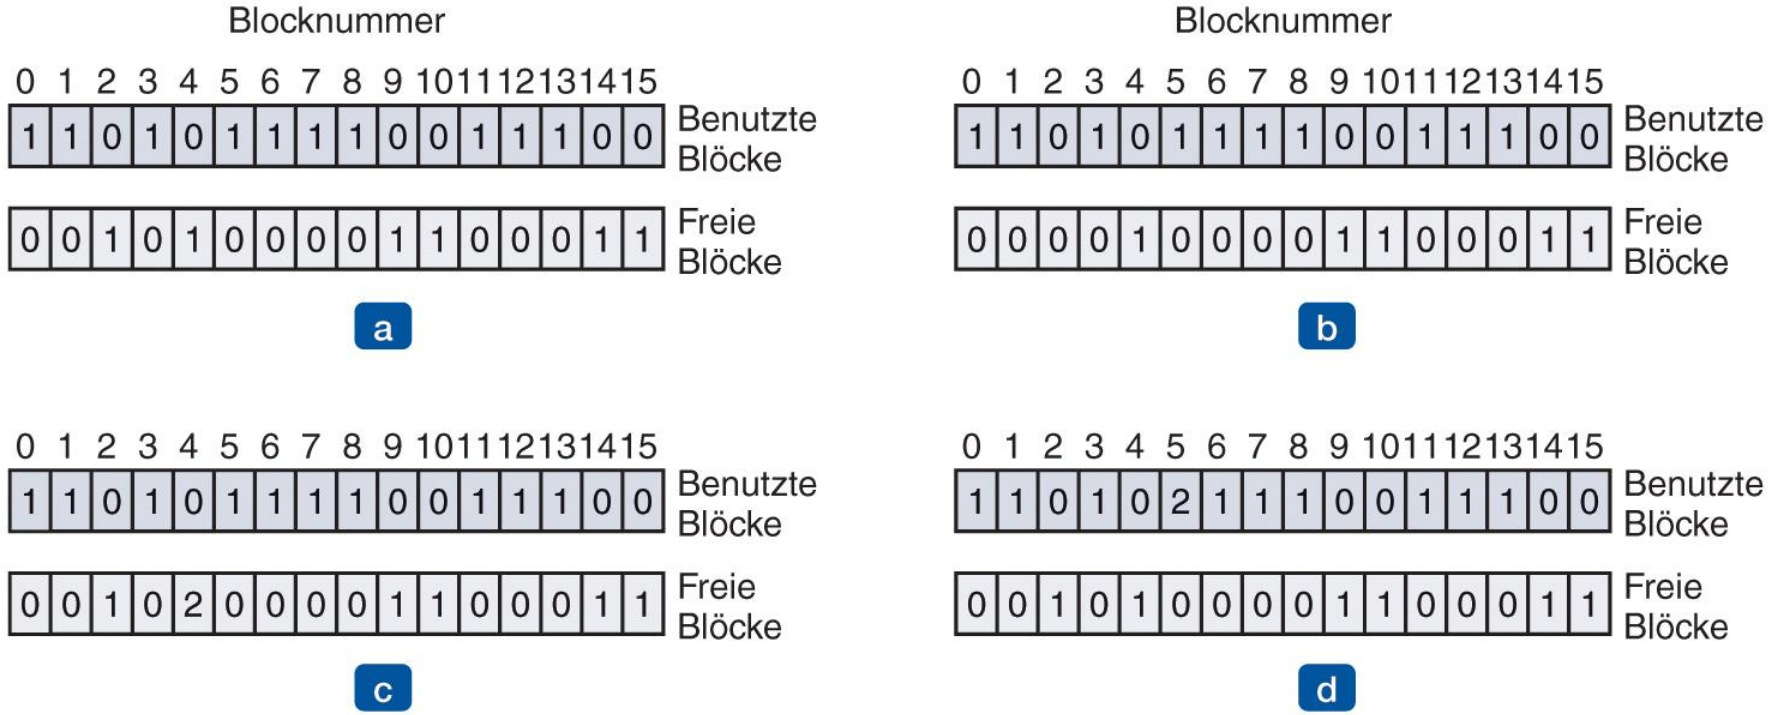
\includegraphics[width=\linewidth]{fsck.png}

\begin{enumerate}[label=\alph*.]
    \item Benutzte und Freie Blöcke sind Konsistent. Alles ist in ordnung.
    \item Es Fehllen Blöcke. Fehlende Blöcke in Freispeicherliste eintragen
    \item Blöcke sind doppelt in Freispeicherliste vorhanden. Freispeicherliste muss
          erneut aufgebaut werden
    \item Blöcke sind Doppelt in Datenliste vorhanden. Desaster!
\end{enumerate}

\subsection{Test der Verzeichnisstruktur}

Soll eine Verzeichnisstruktur getestet werden, So wird eine Tabelle mit je
einem Zähler pro Datei ausgehend vom Wurzelverzeichnis aufgebaut. Für jede
Datie in jedem Verzeichnis wird der Zähler für den I-Node der Datei
inkrementiert. Hard-Links zählen, Soft-Links nicht. Anschließend wird eine
Liste erzeugt, die durch I-Node-Nummern indiziert wird und die Anzahl der auf
diesem I-Node zeigenden Verzeichnisse enthält. Nummern werden mit den Zählern
der Links, die in dem I-Node selbst gespeichert ist, verglichen.

Wenn die Linkzählertabelle gleich dem Tabellenzähler ist, ist alles in ordnung.
Ist der Linkzähler größer als der Tabellenzähler, so können I-Nodes nie
gelöscht werden. Es wird Plattenplatz verschwendet, da in keinem Verzeichnis
ein Link auf diese Datei existiert. Der Linkzähler im I-Node wird auf den
korrekten Wert gesetzt. Ist der Linkzähler kleiner als der Tabellenzähler, so
sind mehrere Verzeichniseinträge mit einer Datei verbunden. Wird eine Datei zu
früh gelöscht und in einem Verzeichnis existiert dann noch ein Verweis auf
einen leeren I-Node.

\subsection{Verstehentliches löschen}

Der Benutzer wird vor sich selbst geschützt. Löscht man eine Datei in den
meisten Betriebssystemen, so wird nur ein Bit im Verzeichnis oder in der I-Node
gesetzt, dass die Datei überschrieben werden darf. Hilfsprogramme können die
Datei zurück holen. Windows besitzt einen Papierkorb, aus dem die Datei noch
herausgeholt werden kann.

\subsection{Performanz eines Dateisystems}

Ein Plattenzugriff ist viel langsamer als ein Speicherzugriff. Zugriffszeit auf
ein 32-Bit Wort im RAM dauert nur ca. 10ns. Auf ein 32-Bit Wort auf der platte
dauert dies ca. 10ms. Um dieses Problem zu umgehen, muss die Plattenperformance
erhöht werden.

\subsubsection{Cashing}

Um die Zugriffszeit der Plattenblöcke zu verringern, existiert ein
\textbf{Block-Cash}. In diesem ist eine Sammlung von Blöcken im Speicher, die
auf die Platte gehören. Bei Leseanfragen wird überprüft, ob der Block im Cashe
ist. Ist dieser im cash, kann er einfach entnommen werden. Andernfalls muss er
von der Platte geholt werden. Er wird dann im Cashe abgelegt. Der Zugriff auf
den Cashe funktioniert über eine Hashfunktion. Das Ergebnis steht in einer
Hashtabelle. Ist der Cashe voll, so müssen Blöcke entfernt werden.

\subsubsection{Probleme}

Stürzt das Dateisystem ab, so kann es zu Dateisysteminkonsistenz kommen.
Modifizierte für die Dateikonsistenz wichtige Blöcke müssen forciert
zurückgeschrieben werden, wie z.B. I-Node Blöcke, indirekte Blöcke,
Verzeichnisblöcke etc.

Auch Modifizierte Blöcke müssen aus dem Cashe zurück geschrieben werden. Unter
UNIX läuft das Programm \texttt{update} als Dämon im Huntergrund und schreibt
alle 30 Sekunden per Fehel \texttt{sync} die modifizierten Blöcke zurück. Der
Nachteil hier ist, dass das entfernen einer Platte aus dem Laufwerk oft zu
Datenverlust führt oder nicht so einfach funktioniert. Unter Windows wird jeder
modifizierte Block direkt auf die Platte geschrieben. Der Nachteil hier ist,
dass für jede kleine Änderung ein Plattenzugriff erfolgt.

